\documentclass{article}
\usepackage[utf8]{inputenc}
%\usepackage[]{babel}
\usepackage{amsmath} % 
\usepackage{amsfonts}
\usepackage{indentfirst}
\usepackage{graphicx}
\usepackage{makeidx}
\usepackage{hyperref} % Para hiperlinks e urls
\usepackage[usenames,dvipsnames]{color}

% Para os listing (codigos fontes)
\usepackage{listings} 
% Configuracao do estilo dos listing (cola cor e outras coisas)
% From here: https://gist.github.com/eyliu/120689

% This is the color used for MATLAB comments below
\definecolor{MyDarkGreen}{rgb}{0.0,0.4,0.0}
% \definecolor{backcolour}{rgb}{0.95,0.95,0.92}
% \definecolor{backcolour}{rgb}{1,0.8,0.9}
\definecolor{backcolour}{rgb}{1,0.94,0.96}

% For faster processing, load Matlab syntax for listings
\lstloadlanguages{C}%
\lstset{language=C,  
    backgroundcolor=\color{backcolour},
% Use MATLAB
        frame=single,                           % Single frame around code
        basicstyle=\small\ttfamily,             % Use small true type font
        keywordstyle=[1]\color{Magenta}\bfseries,        % MATLAB functions bold and blue
        keywordstyle=[2]\color{Purple},         % MATLAB function arguments purple
        keywordstyle=[3]\color{Blue}\underbar,  % User functions underlined and blue
        identifierstyle=,                       % Nothing special about identifiers
                                                % Comments small dark green courier
        commentstyle=\usefont{T1}{pcr}{m}{sl}\color{MyDarkGreen}\small,
        stringstyle=\color{Purple},             % Strings are purple
        showstringspaces=false,                 % Don't put marks in string spaces
        tabsize=5,                              % 5 spaces per tab
        %
        %%% Put standard MATLAB functions not included in the default
        %%% language here
        morekeywords={xlim,ylim,var,alpha,factorial,poissrnd,normpdf,normcdf, audioread, audiowrite, resample},
        %
        %%% Put MATLAB function parameters here
        morekeywords=[2]{on, off, interp},
        %
        %%% Put user defined functions here
        morekeywords=[3]{FindESS, homework_example, tonegen, dtmfgen, halfsp, doublesp, gera_eco},
        %
        morecomment=[l][\color{Blue}]{...},     % Line continuation (...) like blue comment
        numbers=left,                           % Line numbers on left
        firstnumber=1,                          % Line numbers start with line 1
        numberstyle=\tiny\color{Blue},          % Line numbers are blue
        stepnumber=5                            % Line numbers go in steps of 5
        }

\renewcommand{\lstlistingname}{Code}% Modifica o nome 'Listing' para 'Código'

% Includes a MATLAB script.
% The first parameter is the label, which also is the name of the script
%   without the .m.
% The second parameter is the optional caption.
\newcommand{\matlabscript}[2]
  {\begin{itemize}\item[]\lstinputlisting[caption=#2,label=#1]{#1.m}\end{itemize}}

% Coloca nome 'apendice' no sumario
\usepackage[titletoc]{appendix}

% Modifica 'appendices' para 'apendices'
\renewcommand{\appendixpagename}{Appendix}


% Formatacao das margens do texto
\usepackage[top= 3.5cm, left= 3.5cm, right= 3cm, bottom= 3cm]{geometry} 

\usepackage{tocloft}
\renewcommand{\cftsecleader}{\cftdotfill{\cftdotsep}} % coloca pontos no sumario

%Import the natbib package and sets a bibliography  and citation styles
\usepackage[square,numbers]{natbib}
% \bibliographystyle{abbrvnat}
% \setcitestyle{authoryear,open={((},close={))}}

\title{\vspace{-3cm}Federal Institute of Santa Catarina\\
Florianópolis Campus\\
Electronic Engineer \\
\vspace{7cm}
\textbf{Complexity of Implementation}\\
\vspace{1cm}
}
\author{Jhonatan de Freitas Lang \\
\vspace{8cm}}
\date{March 20, 2019}
\makeindex
%\pagenumbering{Roman} % Start roman numbering

\begin{document}
\begin{titlepage}
\clearpage\maketitle
\thispagestyle{empty}
\end{titlepage}
%\newpage
\pagenumbering{roman}
\tableofcontents
\newpage
\pagenumbering{arabic} % Switch to normal numbers
%------------------------------------------------------------------------
\section{Introduction}
%------------------------------------------------------------------------
This report aims to present the resolution of Activity 1 of the discipline Digital Signals Processing II. 
The estimates and implementations were done using a AVR platform, programmed in Assembly language.  The results are presented through graphs, source codes of programs made, images captured in the simulation software Proteus Isis and images captured from the oscilloscope.

%------------------------------------------------------------------------
\section{Objectives}
%------------------------------------------------------------------------
\begin{itemize}
\item Using the datasheet information about instructions of the chosen platform, estimate the number of cycles and the number of cycles per tap that takes to implement the intern product. 
\begin{equation}\label{eq:interProduct}
W = \sum_{k=0}^{N-1} x[k]y[k]
\end{equation}
With the value of N being 2 and 8. Consider that the signal is already in memory;
\item Implement on the simulation software and do the comparison between simulation and estimate;
\item Implement on the platform, check with an oscilloscope, plot a graph with N in x and cycles/tap in y for N = 2, 4, 8, 16, 32, 64.
\end{itemize}
%------------------------------------------------------------------------
\section{Estimating the complexity}
%------------------------------------------------------------------------
Opting to use the ATmega328P operating at 16MHz to perform this activity, for reasons such as availability and compatibility with the requirement to be an 8-bit platform.

After the sketch of the sum algorithm, was searched in the microcontroller datasheet\cite{AVR}. the needed assembly instructions and the clock cycles required to execute.

Given the appropriate considerations for the initial memory state, the code cutout below is the part of the main loop  where the number of clock cycles is counted.

\matlabscript{./codigos/loopSum}{Main Loop }

Since the number of cycles in the chosen implementation can be calculated by:
\begin{equation}\label{eq:cyclesNumber}
cycles(N) = N\cdot(2+2+2+1+1+2) + 2 - 1
\end{equation}
\begin{equation}\label{eq:cyclesNumberS}
cycles(N) = N\cdot10 + 1
\end{equation}

The table \ref{tab:Est_N} shows the estimates of total cycles, cycles/tap and runtime with ATmega328p operating at 16 MHz for N = 2, 4, 8, 16, 32, 64. 

\begin{table}[!ht]
\begin{center}
\caption{Estimate complexity}
\begin{tabular}{|c|c|c|c|c|}
\hline
\textbf{N} & \textbf{Total cycles} & \textbf{Cycles/Tap} & \textbf{Runtime} \\
\hline
\textbf{2}  & 21  & 10.5      & 1.3125E-06  \\
\textbf{4}  & 41  & 10.25     & 2.5625E-06  \\
\textbf{8}  & 81  & 10.125    & 5.0625E-06  \\
\textbf{16} & 161 & 10.0625   & 1.00625E-05 \\
\textbf{32} & 321 & 10.03125  & 2.00625E-05 \\
\textbf{64} & 641 & 10.015625 & 4.00625E-05 \\
\hline
\end{tabular}
\label{tab:Est_N}
\end{center}
\end{table}


The graph \ref{fig:Est_NxTap}. shows a relation N x Cycles/Tap that expect to be found

\begin{figure}[!ht]
\centering
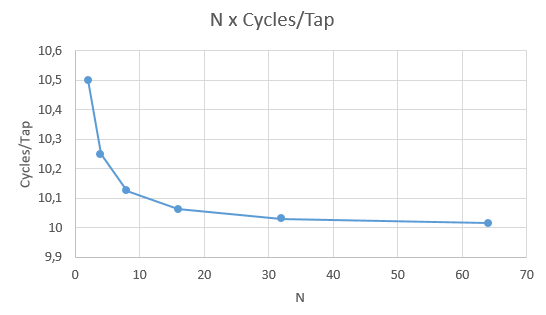
\includegraphics[width=0.7\textwidth]
{./figuras/Estimate_NxTap.png}
\caption{Estimate N x Cycles/Tap}
\label{fig:Est_NxTap}
\end{figure}


%------------------------------------------------------------------------
\section{Simulation}
%------------------------------------------------------------------------
After estimate the number of cycles to implement de intern product. the microcontroller was simulated on the software Proteus Isis. An output pin of the microcontroler was configured to switch to high logic level at the beginning of the sum loop and to low logic level after breack the loop and save the value in the memory. This way is possible to see the through an oscilloscope the time window where the operation occurs. 

the figures \ref{fig:S_N_2} and \ref{fig:S_N_4} are prints of the oscilloscope of simulator, with values of N = 2 and N = 8.

\begin{figure}[!ht]
\centering
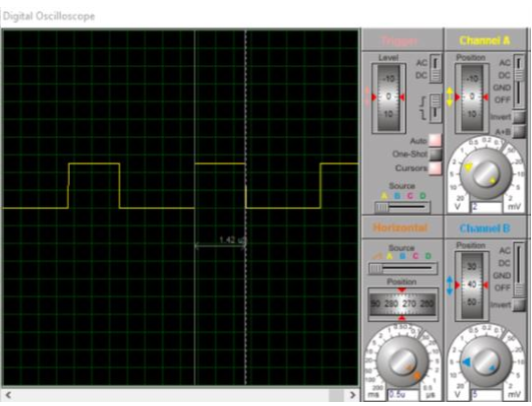
\includegraphics[width=0.7\textwidth]
{./figuras/S_N_2.PNG}
\caption{Runtime to N = 2 on Simulation}
\label{fig:S_N_2}
\end{figure}

\begin{figure}[!ht]
\centering
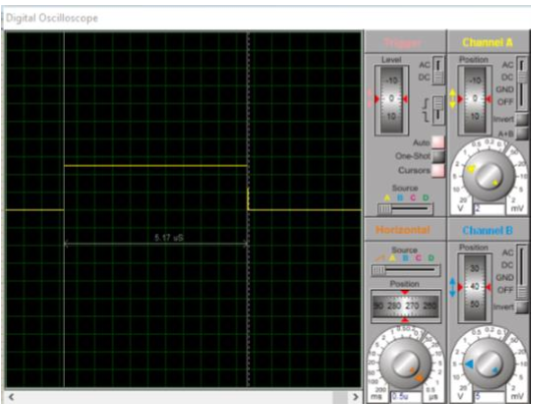
\includegraphics[width=0.7\textwidth]
{./figuras/S_N_4.PNG}
\caption{Runtime to N = 4 on Simulation}
\label{fig:S_N_4}
\end{figure}

Getting the runtime to N values was possible to do the table \ref{tab:S_C}.


\begin{table}[!ht]
\begin{center}
\caption{Simulate complexity}
\begin{tabular}{|c|c|c|c|c|}
\hline
\textbf{N} & \textbf{Total cycles} & \textbf{Cycles/Tap} & \textbf{Runtime} \\
\hline
\textbf{2}  & 22.72  & 11.36     & 1.42E-06  \\
\textbf{4}  & 42.72  & 10.68     & 2.67E-06  \\
\textbf{8}  & 82.72  & 10.34     & 5.17E-06  \\
\textbf{16} & 163.84 & 10.24     & 1.2E-05 \\
\textbf{32} & 323.84 & 10.12     & 2.2E-05 \\
\textbf{64} & 643.04 & 10.05     & 4.2E-05 \\
\hline
\end{tabular}
\label{tab:S_C}
\end{center}
\end{table}


As we can see on the graph \ref{fig:S_NxTap}, the cycles/tap values are quickly greater than estimate values. Probably because the delay times  to switch the output pin was not considered. But as the value of N increases, this graph also tends to 10 Cycles / Tap.

\begin{figure}[!ht]
\centering
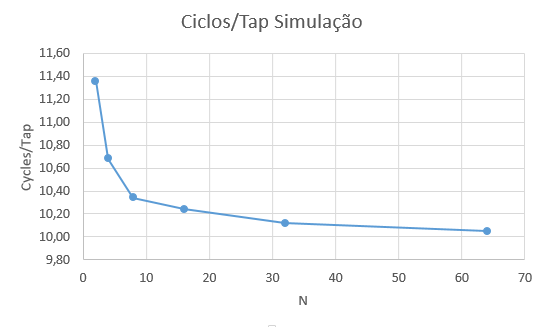
\includegraphics[width=0.7\textwidth]
{./figuras/S_NxTAP.PNG}
\caption{Simulated NxCycles/Tap}
\label{fig:S_NxTap}
\end{figure}


%------------------------------------------------------------------------
\section{Pratice}
%------------------------------------------------------------------------

As implemented in the simulation, the circuit was implemented in practice. Being the code burned at a ATmega328P and the output pin was watched  for an bench oscilloscope.

The figures \ref{fig:P_N_2} and \ref{fig:P_N_64} are prints of the bench oscilloscope, with values of N = 2 and N = 64.

\begin{figure}[!ht]
\centering
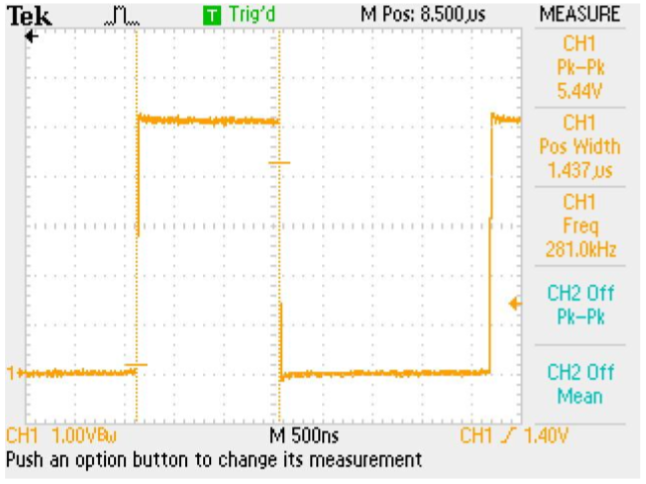
\includegraphics[width=0.7\textwidth]
{./figuras/P_N_2.PNG}
\caption{Runtime to N = 2 on Pratice}
\label{fig:P_N_2}
\end{figure}

\begin{figure}[!ht]
\centering
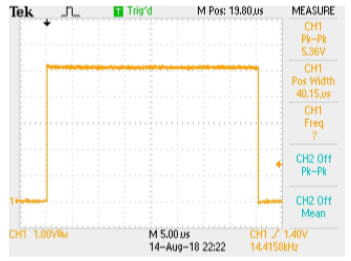
\includegraphics[width=0.7\textwidth]
{./figuras/P_N_64.PNG}
\caption{Runtime to N = 64 on Pratice}
\label{fig:P_N_64}
\end{figure}

Changing the N value and reading the output pin was filled out the table \ref{tab:P_C}

\begin{table}[!ht]
\begin{center}
\caption{Pratice complexity}
\begin{tabular}{|c|c|c|c|c|}
\hline
\textbf{N} & \textbf{Total cycles} & \textbf{Cycles/Tap} & \textbf{Runtime} \\
\hline
\textbf{2}  & 22.992  & 11.496  & 1.437E-06  \\
\textbf{4}  & 42.976  & 10.744  & 2.686E-06  \\
\textbf{8}  & 82.944  & 10.368  & 5.184E-06  \\
\textbf{16} & 162.88  & 10.180  & 1.018E-05 \\
\textbf{32} & 322.72  & 10.085  & 2.017E-05 \\
\textbf{64} & 642.40  & 10.038  & 4.015E-05 \\
\hline
\end{tabular}
\label{tab:P_C}
\end{center}
\end{table}


Note that the values of the practical table, within a minimum tolerance, are the same as in the theoretical table, just as the graph obtained can be read in the same way, look the figure\ref{fig:P_NxTap}


\begin{figure}[ht]
\centering
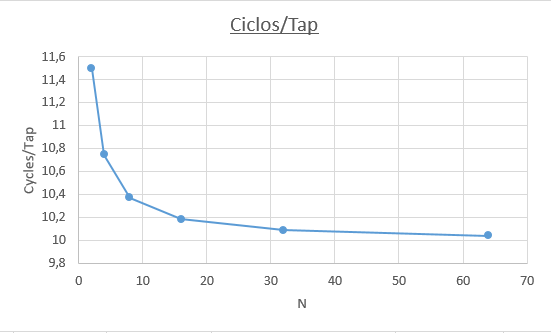
\includegraphics[width=0.7\textwidth]
{./figuras/P_NxTAP.PNG}
\caption{Pratice NxCycles/Tap}
\label{fig:P_NxTap}
\end{figure}


%------------------------------------------------------------------------
\section{Conclusion}
%------------------------------------------------------------------------
Although a chosen loop implementation has a higher cost with an overhead than a sequential session of all operations, is easier than a sequential implementation as complexity N increases,also more compact .

We can also observe that the overhead is fixed and how it is diluted with the increment of N.

\bibliographystyle{plainnat}
\bibliography{bibliografia}

%------------------------------------------------------------------------
% \appendix
%------------------------------------------------------------------------
\begin{appendices}
\appendix
\appendixpage
\section{Implemented Code} \label{ape:fullCode}
\matlabscript{./codigos/Code1}{Full Code}

\end{appendices}

\end{document}